\documentclass[aspectratio=169, 10pt]{beamer}

\usepackage[T1]{fontenc}
\usepackage[utf8]{inputenc}
\usepackage[polish]{babel}
\usepackage{lmodern}
\usepackage{graphicx}
\usepackage{booktabs}
\usepackage{amsmath}

\usetheme{metropolis}
\metroset{block=fill, progressbar=frametitle, numbering=fraction}

\definecolor{pwblue}{RGB}{27, 54, 93}
\definecolor{pwaccent}{RGB}{180, 45, 45}
\setbeamercolor{palette primary}{bg=pwblue, fg=white}
\setbeamercolor{progress bar}{fg=pwaccent, bg=pwblue!25}
\setbeamercolor{alerted text}{fg=pwaccent}

\title{Symulacja i analiza rozkładów cząstek w zderzeniach $pp$ przy $\sqrt{s} = 13{,}6\text{ TeV}$}
\subtitle{Zadanie wstępne z analizy danych (Pythia 8 + ROOT)}
\author{Krzysztof Wojczakowski}
\institute{Wydział Matematyki i Nauk Informacyjnych, Politechnika Warszawska}
\date{}

\begin{document}

% -----------------------------------------------------------------------------
\begin{frame}[plain]
  \titlepage
\end{frame}

% -----------------------------------------------------------------------------
\begin{frame}{Parametry symulacji i analizy}
  \begin{columns}[T, onlytextwidth]
    \begin{column}{0.52\textwidth}
      \textbf{Generacja zdarzeń (Pythia 8):}
      \begin{itemize}
        \item Zderzenia $pp$ przy $\sqrt{s} = 13{,}6\text{ TeV}$
        \item Tryb \texttt{SoftQCD:all = on} (minimum bias)
        \item $100\,000$ zdarzeń, stały seed (\texttt{12345})
        \item Tylko cząstki stanu końcowego (\texttt{isFinal()})
      \end{itemize}

      \vspace{0.5em}
      \textbf{Analizowane grupy (32 histogramy):}
      \begin{itemize}
        \item \texttt{all} -- wszystkie cząstki końcowe
        \item \texttt{ch} -- wszystkie cząstki naładowane ($q \neq 0$)
        \item $\pi^\pm$ ($\pm 211$), $K^\pm$ ($\pm 321$), $p,\bar{p}$ ($\pm 2212$)
      \end{itemize}
    \end{column}

    \begin{column}{0.45\textwidth}
      \textbf{Zakresy histogramów (\texttt{analysis.root}):}
      \vspace{0.5em}
      \begin{table}
        \centering
        \small
        \begin{tabular}{@{}lcc@{}}
          \toprule
          Zmienna & Zakres & Biny \\
          \midrule
          Krotność $N$ & $[0,\; 400)$ & 400 \\
          Pęd poprzeczny $p_T$ & $[0,\; 10)\text{ GeV}$ & 100 \\
          Pseudorapidity $\eta$ & $[-5,\; 5)$ & 100 \\
          Kąt azymutalny $\phi$ & $[0,\; \pi]\text{ rad}$ & 64 \\
          \bottomrule
        \end{tabular}
      \end{table}

      \vspace{0.4em}
      \footnotesize
      Kąt $\phi$ z Pythii należy do $(-\pi, \pi]$, dlatego w analizie użyto $|\phi|$, aby zmieścić cały rozkład w $[0, \pi]$ bez odrzucania połowy danych.
    \end{column}
  \end{columns}
\end{frame}

% -----------------------------------------------------------------------------
\begin{frame}{Krotność cząstek na zdarzenie ($N$)}
  \begin{center}
    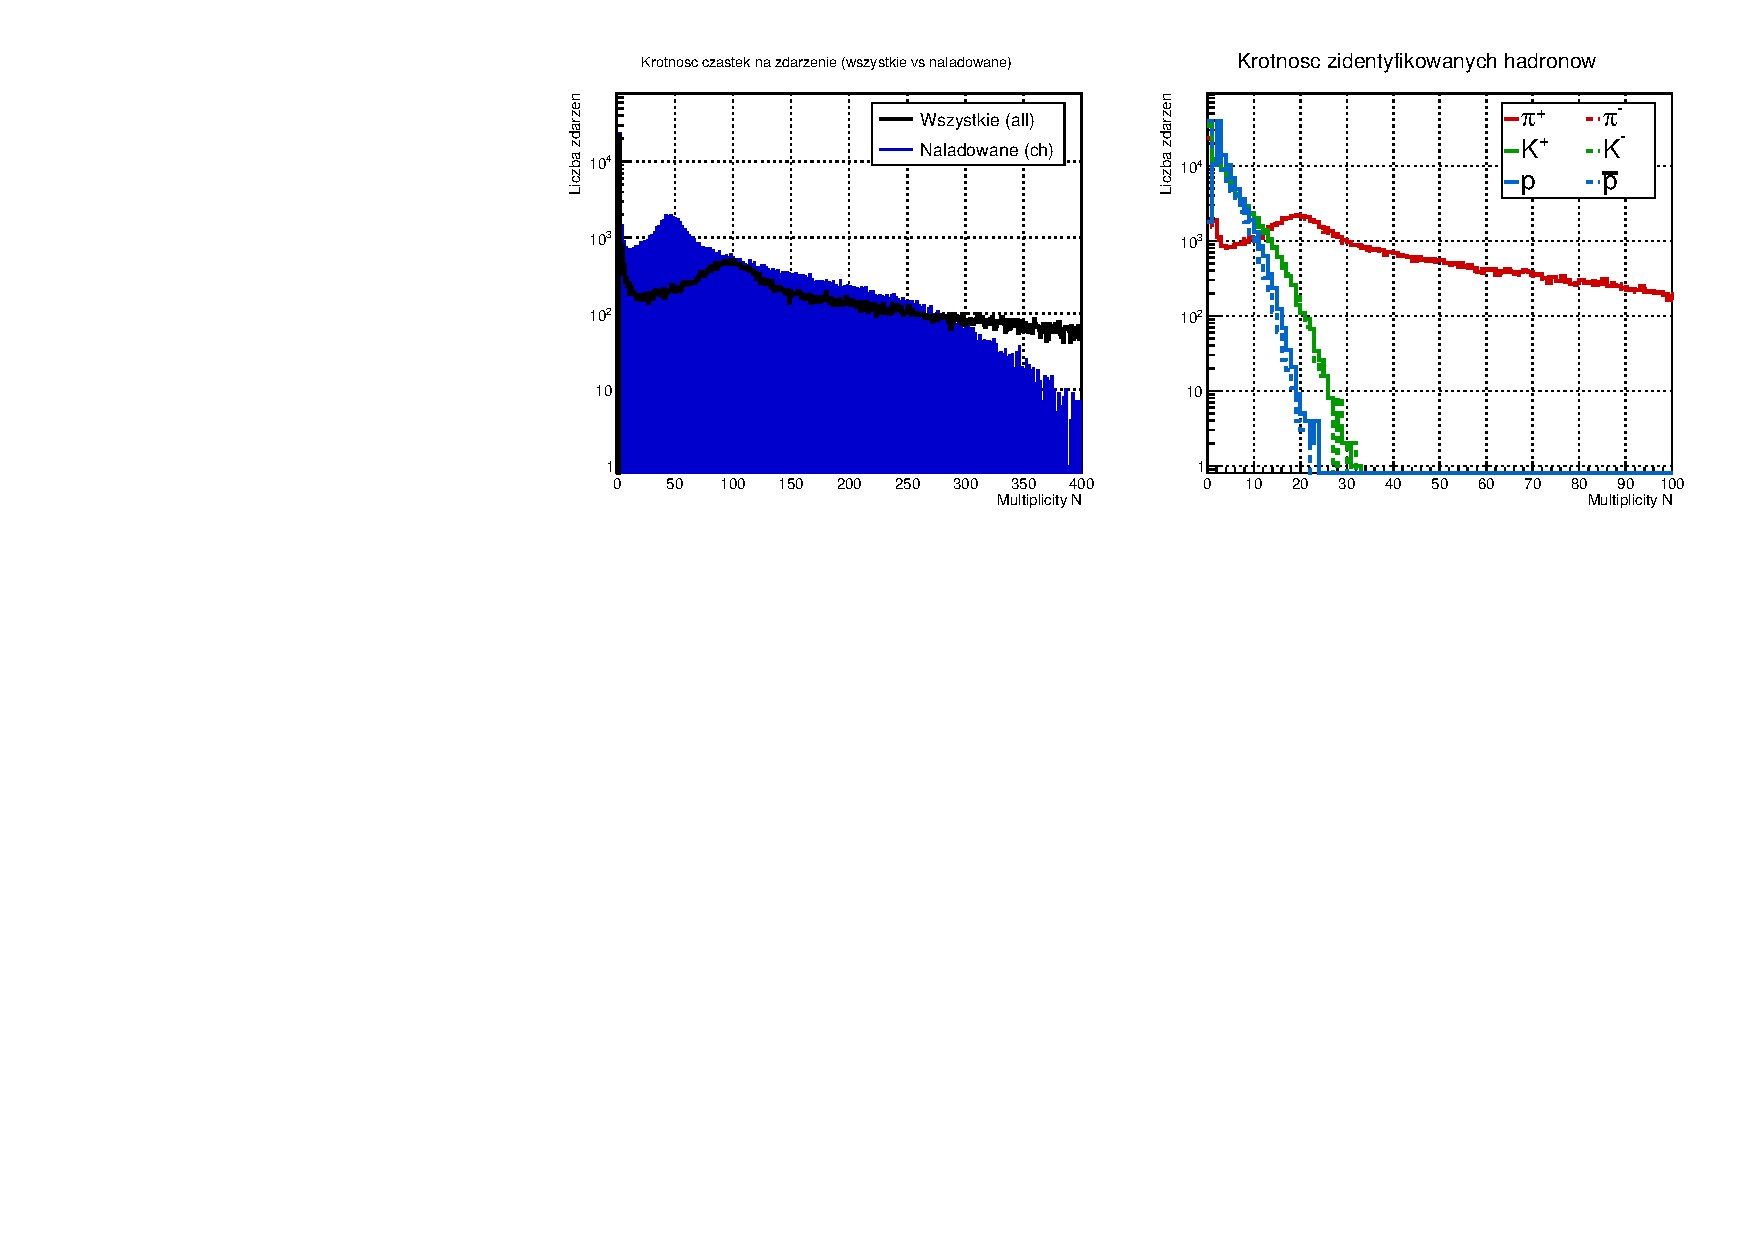
\includegraphics[page=1, width=0.98\textwidth, height=0.63\textheight, keepaspectratio]{plots/all_distributions.pdf}
  \end{center}
  \vspace{-0.4em}
  \small
  \begin{itemize}
    \item \textbf{Po lewej:} Liczba wszystkich cząstek (średnio ok.\ $149$) i naładowanych (średnio ok.\ $71$). Liczba cząstek naładowanych jest zawsze parzysta (nieparzyste biny $= 0$), a pik w $N = 2$ pochodzi ze zderzeń, w których dwa protony po prostu się odbijają.
    \item \textbf{Po prawej:} Najwięcej powstaje pionów ($\pi^\pm$), a znacznie mniej kaonów ($K^\pm$) oraz protonów i antyprotonów ($p, \bar{p}$).
  \end{itemize}
\end{frame}

% -----------------------------------------------------------------------------
\begin{frame}{Rozkład pędu poprzecznego ($p_T$)}
  \begin{center}
    \includegraphics[page=2, width=0.98\textwidth, height=0.63\textheight, keepaspectratio]{plots/all_distributions.pdf}
  \end{center}
  \vspace{-0.4em}
  \small
  \begin{itemize}
    \item \textbf{Po lewej:} Większość cząstek ma mały pęd poprzeczny (poniżej $1\text{--}2\text{ GeV}$); im większe $p_T$, tym szybciej spada liczba cząstek (skala logarytmiczna).
    \item \textbf{Po prawej:} W całym zakresie pędów najliczniejsze są najlżejsze piony ($\pi^\pm$), natomiast kaonów ($K^\pm$) i protonów ($p, \bar{p}$) jest wyraźnie mniej.
  \end{itemize}
\end{frame}

% -----------------------------------------------------------------------------
\begin{frame}{Rozkład pseudorapidity ($\eta$)}
  \begin{center}
    \includegraphics[page=3, width=0.98\textwidth, height=0.63\textheight, keepaspectratio]{plots/all_distributions.pdf}
  \end{center}
  \vspace{-0.4em}
  \small
  \begin{itemize}
    \item \textbf{Symetria:} Rozkład jest symetryczny względem $\eta = 0$, ponieważ zderzamy dwa takie same protony o tej samej energii.
    \item \textbf{Kształt:} Widać lekkie obniżenie na środku (w okolicach $\eta = 0$) i maksima przy $|\eta| \approx 2$. Cząstki naładowane stanowią ok.\ połowy wszystkich cząstek.
  \end{itemize}
\end{frame}

% -----------------------------------------------------------------------------
\begin{frame}{Rozkład kąta azymutalnego ($\phi$)}
  \begin{center}
    \includegraphics[page=4, width=0.98\textwidth, height=0.63\textheight, keepaspectratio]{plots/all_distributions.pdf}
  \end{center}
  \vspace{-0.4em}
  \small
  \begin{itemize}
    \item \textbf{Równomierność:} Rozkład jest płaski w całym zakresie $[0, \pi]$ -- cząstki rozlatują się tak samo w każdym kierunku wokół osi wiązki.
    \item \textbf{Po prawej:} Widać, że protonów ($p$) jest nieco więcej niż antyprotonów ($\bar{p}$), co wynika z tego, że na wejściu zderzamy dwa protony.
  \end{itemize}
\end{frame}

% -----------------------------------------------------------------------------
\begin{frame}{Podsumowanie wyników}
  \begin{columns}[T, onlytextwidth]
    \begin{column}{0.58\textwidth}
      \begin{table}
        \centering
        \footnotesize
        \setlength{\tabcolsep}{4.5pt}
        \begin{tabular}{@{}lrrr@{}}
          \toprule
          Kategoria & Liczba cząstek & Średnie $N$ & Średnie $p_T$ [GeV] \\
          \midrule
          Wszystkie (\texttt{all}) & $14\,889\,356$ & $148{,}89$ & $0{,}40$ \\
          Naładowane (\texttt{ch}) & $7\,137\,540$ & $71{,}38$ & $0{,}51$ \\
          \midrule
          $\pi^{+}$ & $2\,954\,507$ & $29{,}55$ & $0{,}48$ \\
          $\pi^{-}$ & $2\,902\,645$ & $29{,}03$ & $0{,}48$ \\
          $K^{+}$ & $325\,065$ & $3{,}25$ & $0{,}68$ \\
          $K^{-}$ & $316\,213$ & $3{,}16$ & $0{,}68$ \\
          $p$ & $342\,945$ & $3{,}43$ & $0{,}63$ \\
          $\bar{p}$ & $203\,698$ & $2{,}04$ & $0{,}78$ \\
          \bottomrule
        \end{tabular}
      \end{table}
    \end{column}

    \begin{column}{0.38\textwidth}
      \textbf{Zrealizowane pliki:}
      \small
      \begin{itemize}
        \item \texttt{generate.cc} -- generacja $100\,000$ zdarzeń w Pythia 8.
        \item \texttt{analyze.cc} -- utworzenie 32 histogramów w \texttt{analysis.root}.
        \item \texttt{draw\_plots.C} -- wygenerowanie wykresów PNG i PDF.
      \end{itemize}
    \end{column}
  \end{columns}
\end{frame}

\end{document}
